\documentclass[letterpaper,10pt,twocolumn]{article}
\usepackage{usenix}

\usepackage{footmisc}
%\usepackage[T1]{fontenc}
%\usepackage{fontspec}
%\setmainfont{Times New Roman}
\usepackage{times}
\usepackage{xcolor}
\usepackage{xspace}
\usepackage{type1cm}
\usepackage{boxedminipage}
\usepackage{pifont}
\usepackage{pseudocode}
\usepackage{multirow}
\usepackage{tabularx}
\usepackage{caption}
\usepackage{subcaption}
\usepackage{graphicx}
\usepackage{savetrees}  % This is awesome wow!
\usepackage{geometry}
\usepackage{titlesec}
\usepackage{titling}
\usepackage{leading}
\usepackage{amsmath}
\usepackage[titletoc,title]{appendix}

% jvesuna: Section formatting. Enable to make them big.
\usepackage{sectsty}
\sectionfont{\fontsize{14}{12}\selectfont}
\subsectionfont{\fontsize{12}{12}\selectfont}

\setlength{\droptitle}{-0.56in}

%\usepackage{relsize}
%\titlelabel{\larger\larger\thetitle\quad\aftergroup\larger\aftergroup\larger}

%\linespread{1.0527}

%\titlespacing{\section}{0cm}{0cm}{0cm}
%\titleformat{\section} {\itshape\normalsize}{\theparagraph}{1em}{#1}
%\titlespacing\section{0pt}{-12pt plus 4pt minus 2pt}{-15 pt plus 2pt minus 2pt}

%\usepackage{savetrees}
%\setlength{\belowcaptionskip}{-10pt}

%\geometry{lmargin=0.5in, rmargin=0.5in, tmargin=0.75in, bmargin=0.75in}

\geometry{lmargin=1in, rmargin=1.02in, tmargin=1in, bmargin=0.91in}


\definecolor{MyDarkBlue}{rgb}{0,0.08,0.45}
\usepackage[pdftex]{hyperref}
\hypersetup{
  colorlinks,%
  citecolor=MyDarkBlue,%
  filecolor=MyDarkBlue,%
  linkcolor=MyDarkBlue,%
  urlcolor=MyDarkBlue
}
\usepackage{fixltx2e}
\usepackage{textgreek}
\usepackage[sort]{cite}

% ---------------- Notes: -----------------------

\newcommand{\tbd}[1]{{\bf [[TBD: {#1}]]}}
\newcommand{\eat}[1]{}

\newcommand{\num}[1]{{\color{red}\bf {#1}}}

\newcommand*{\figuretitle}[1]{
{\centering
    \textbf{#1}
    %\vspace{0.7in}
    \par\medskip}
}

\newcommand{\colin}[1]{{\color{red}\bf CS: {#1}}}
\newcommand{\scott}[1]{{\color{purple}\bf SS: {#1}}}
\newcommand{\arvind}[1]{{\color{brown}\bf AK: {#1}}}
\newcommand{\jamshed}[1]{{\color{blue}\bf JV: {#1}}}

\setlength{\footskip}{0.6in}
%\newcommand{\colin}[1]{}
%\newcommand{\scott}[1]{}

\sloppy
\title{\vspace{0.04in}Caching Doesn't Improve Mobile Web Performance (Much)}

\DeclareRobustCommand{\authorthing}{
\vspace{-0.5in}
\rm Jamshed Vesuna$^\dagger$
\and \rm Colin Scott$^\dagger$
\and \rm Michael Buettner$^\diamond$
\and \rm Michael Piatek$^\diamond$
\and \rm  Arvind Krishnamurthy$^\star$
\and \rm Scott Shenker$^\dagger$$^\ddagger$
\and {\begin{tabular}{cccc}
$^\dagger$UC Berkeley & $^\ddagger$ICSI & $^\diamond$Google & $^\star$University of Washington
\end{tabular}}
}
\author{\authorthing}

%\titlespacing*{\section}{0pt}{1pt plus 1pt minus 3pt}{1pt plus 1pt minus 3pt}
%\titlespacing*{\subsection}{0pt}{1pt plus 1pt minus 3pt}{1pt plus 1pt minus 3pt}

\begin{document}
   \date{}
   \maketitle
   \thispagestyle{empty}

\leading{12pt}
\setlength{\textfloatsep}{10pt plus 1pt minus 10pt} % To reduce space after figures

\abstract{A recent NSDI paper~\cite{flywheel} reported a counterintuitive result:
increasing the cache hit ratio of their HTTP proxy from 22\% to 32\% only improved median page load time for mobile clients by 1-2\%.
%In their NSDI paper~\cite{flywheel}, Google reported a counterintuitive result: increasing the cache hit ratio of their Flywheel HTTP proxy from 22\% to 32\% only improved median page load time for mobile clients by 1-2\%.
Here, we seek to understand why improved caching had such a negligible effect on mobile performance. 
We reproduced these results in a controlled, mobile environment and observed comparable reductions of 1\% in the median case for a 50\% increase in cache hit ratio.
Further, we show that with a perfect cache hit ratio, desktop page load times are improved notably by 34\% compared to no caching, but mobile page load times only improve by 13\% in the median case.
We demonstrate that CPU speed is the key bottleneck preventing mobile devices from benefiting from web caching.

%\colin{when we get the partial caching results, you might want to replace the 35\%, 13\% statistics with the partial caching reuslts.}

% CS: removing this for now, since it isn't required in the CFP:
%    https://www.usenix.org/conference/atc16/requirements-authors
%\\\\
%\noindent
%\textbf{Keywords:} mobile, web performance, web caching}

\section{Introduction}
\label{sec:intro}
\label{intro}
%With the increase in mobile Internet traffic, there is a larger emphasis on methods of improving web performance for mobile devices.
Web caching is widely used to reduce network link utilization, decrease server load and data usage, improve reliability for origin web servers, and improve latency for end hosts.
Here, we focus exclusively on web caching's effect on latency, as measured by web page load time.

Flywheel~\cite{flywheel}, Google's HTTP proxy for mobile devices, increased
its overall cache hit ratio from 22\% to 32\%, yet observed only a 1--2\% reduction in page load time in the median case.
Here we seek to gain a deeper understanding of why improved caching had such a negligible effect on performance.

% Can we remove this first sentence?
%Our contributions are as follows.
We present a methodology
% Commenting this out because they don't know what WPR and Telemetry are yet.
%based on Web Page Replay~\cite{wpr} and Telemetry~\cite{telemetry}
for evaluating the performance impact of web caching for hypothetical levels of cache hit ratios, in a controlled environment. We use this methodology to compare the effects of partial (hit ratio of 20\% to 30\%) and
perfect caching (hit ratio of 100\%) versus no caching for a set of 400 Alexa web pages~\cite{alexa} on both a mobile device and a desktop browser.

We demonstrate that by increasing the cache hit ratio from 20\% to 30\%, there is only a meager 1\% reduction in mobile web page load time.
Further, we show that with perfect caching, desktop page load times are improved notably by 34\% compared to no caching, but mobile page load times only improve by 13\% in the median case.
We finally show that CPU speed is the key resource bottleneck preventing mobile devices from benefiting significantly from web caching.

Our results suggest that the common wisdom that web caching is a crucial part of web performance optimization may not hold for mobile clients. Content providers may want to reconsider where they focus their efforts, especially as the volume of mobile traffic begins to overtake desktop traffic.

% TODO(cs): attempt to argue that others, besides the Flywheel authors, also
% suffer from the same misconception about web caching's potential benefits?


%\vspace{-0.3in}
\section{Background \& Performance Model}
\label{sec:background}
Both browsers and mobile applications typically load content using the HTTP protocol. When a user directs the browser (or application) to a new URL, the browser's Object Loader fetches the root HTML object, as depicted
in Figure~\ref{fig:network-diagram}. The HTML Parser launches additional
fetch requests for each linked resource within the HTML. In this way, the browser incrementally generates the DOM.
As the page loads, the Rendering component paints the UI.

From the user's perspective, the performance of a website can be defined according to a number of different metrics~\cite{above-the-fold,speed-index}. Here,
we focus on page load time, which is easy to measure
and loosely standardized across browsers~\cite{w3c-onload}.

\textbf{Page Load Time}. Roughly speaking, page load time (PLT) is the elapsed time from the moment a user requests a web page to the moment all resources on the page have been loaded~\cite{page-speed}.
We measure PLT by listening to the browser's Javascript \texttt{onload} event,
which fires in most browsers when all resources have been added to the DOM, and all images,
scripts, links, and sub-frames have finished loading~\cite{w3c-onload}.

%\colin{Need to make clear that certain objects (tasks) are dependent on others. When a task is dependent on another, it must wait until its dependencies (tasks) have completed. E.g., all tasks are dependent on the HTML parsing task for the root HTML)}
%\jamshed{Added this to "Critical Path" section


\textbf{Critical Path}. Web pages are comprised of many objects, such as images, Javascript, CSS, and HTML.
Each of these objects is handled by multiple (possibly concurrent) browser tasks: it must be
fetched, parsed or evaluated, and rendered. We refer to the non-overlapping
delays involved in parsing and rendering an object as its `computational
delay,' and refer to the fetch delay as its `network delay.'

Critical path analysis is a method for analyzing the performance of parallel
processes such as browsers.
Certain load tasks are dependent on others and must wait until their
predecessor tasks have completed. The critical path of a web page is the longest chain of dependent browser tasks such that reducing the length of any task not on the critical
path will not change the page load time~\cite{sarkar1987partitioning}.
In Figure~\ref{fig:plt-diagram}, the network and computational delay for the HTML, CSS, JS, and JPEG
objects determine the PLT. If we were to decrease the delay for loading the
PNG object, the critical path would remain the same, and therefore, the PLT would not change.

%\colin{Should make a clearer definition for `tasks' and `objects'. The web page is composed of multiple objects, each of which must be fetched (1 task), parsed or evaluated (1 task), and rendered (1 task).}

% TODO(cs): say whether it's possible that objects on the critical path can
% overlap or not. I think it is possible, e.g., if HTML is partially loaded,
% the browser can kick of other (dependant) tasks before the HTML has completed
% loading.

\subsection{Performance Model}
\label{subsec:model}

We are now in a position to develop a simple performance model, which we can
use to gain an understanding of caching's effect on PLT.
First, consider the following terms:
%We show the details of how we derive
%this model in the Appendix~\ref{sec:appendix}.

\noindent-- Let $X$ denote a given cache hit ratio. We define cache hit ratio as the fraction
of all objects in a web page that are served by a cache. Note that the maximum
value of $X$ is the fraction of cacheable items on the page, which may be less than 1.

\noindent-- Let $K$ denote the fraction of objects on the critical path that
are cacheable.

\noindent-- Let $N$ denote the summation of network fetch delays for all objects on the
critical path for a cold ($X=0$) page load.
% Why do we need to assume the hit ratio is 0 when we just said K is independent of the hit ratio above?
% Colin: N and C are constants, i.e. their value needs to be set (measured)
% with a fixed value of X. It's convenient and simplest to set the fixed value
% to X to 0, i.e. ensure that the initial page load did not have any cached
% hits. We could set the initial value of X to something else, but 0 is simplest.

\noindent-- Let $C$ denote the summation of computational delays for all
objects on the critical path for a cold ($X=0$) page load.

\noindent-- Let $f(X)$ denote the overlap between computational delay and
network delay on the critical path. Normally, dependent objects on the
critical path should not overlap with each other, except for some cases where the
browser can begin concurrently loading an object
when its predecessor is only partially loaded.
For most purposes, we can treat $f(X)$
as being close to 0.

For simplicity, let us assume that (i) the critical path does not change as we vary the cache hit
ratio, (ii) the probability of an object being in cache is uniform
across all cacheable objects, and (iii) cached items incur zero network delay. The probability of an object
on the critical path incurring a network delay is then:
\begin{align*}
1 - Pr(\text{object is cacheable}) \cdot Pr(\text{cache hit})
\end{align*}

The expected value of the PLT at a given cache hit ratio is therefore:
\begin{align*}
E_{PLT}[X] = C + (1 - K \cdot X) \cdot N - f(X)
\end{align*}

\subsection{Model Fitting}
\label{subsec:model_fitting}


% TODO(cs): show off some predictions we can make with this model.
% TODO(cs): put Figure 13 from WProf here.


%\vspace{-0.3in}
\section{Experimental Apparatus}
\label{sec:apparatus}
\label{setup}
In order to gain a deeper understanding of the performance dynamics outlined in ~\S\ref{subsec:model} and ~\S\ref{subsec:model_fitting}, we need to experimentally evaluate questions about how caching affects PLT in a controlled environment.
%Our goal for the rest of the paper is to gain a deeper understanding of the performance dynamics outlined in the previous section.
%To do so  we need to experimentally evaluate, in a controlled manner, questions about how caching affects performance.
Here, we develop our methodology.
% To achieve our goal, we must address the following challenge:

Our experimental apparatus (publicly available at~\cite{jamshed-telemetry}) makes use of Telemetry~\cite{telemetry} and Web Page Replay (WPR)~\cite{wpr} to measure the effects of parameterized levels of network delays.
Both Telemetry and WPR are part of Chromium~\cite{chromium-source}, the open source components of Google Chrome.
Here, we use the term `browser' interchangeably with Google Chrome.

\textbf{Web Page Replay}. WPR acts as a local DNS and HTTP(S) proxy cache (depicted in Figure~\ref{fig:workflow_diagram}a).
In record mode, WPR forwards HTTP(S) requests to the Internet, and records all requests and responses that it observes, as well as metadata such as observed network delays. From this, Web Page Replay builds a WPR archive (depicted in Figure~\ref{fig:workflow_diagram}b), complete with all HTTP(S) requests, responses, headers, data, and network delays. % the last part of this sentence is somewhat redundant.

In replay mode, the WPR proxy responds to HTTP(S) requests with the responses saved in the archive, or a 404 error response if the corresponding response is not saved in the archive.
We configure WPR to send the matching response and data only after sleeping for the time duration originally observed as the network delay between the origin and the WPR proxy (while it was in record mode). Here, WPR is emulating an edge cache rather than a browser cache.

\textbf{Telemetry}. Telemetry (Figure~\ref{fig:workflow_diagram}c) is a browser performance testing framework, which orchestrates the behavior of the browser and WPR.
We use Telemetry to control one of two browsers. The first is a desktop version of Google Chrome running within a virtual machine (specifications in ~\ref{specs}). The second is a mobile version of Google Chrome running on a USB-tethered mobile device.
We use Telemetry to load requested URLs in the browser (as if the user is entering URLs into the omnibox) and passively measuring PLT.
\subsection{Workflow} \label{workflow}
\begin{figure}[t]
    \hspace{-10pt}
    \figuretitle{Experimental Apparatus Workflow}
    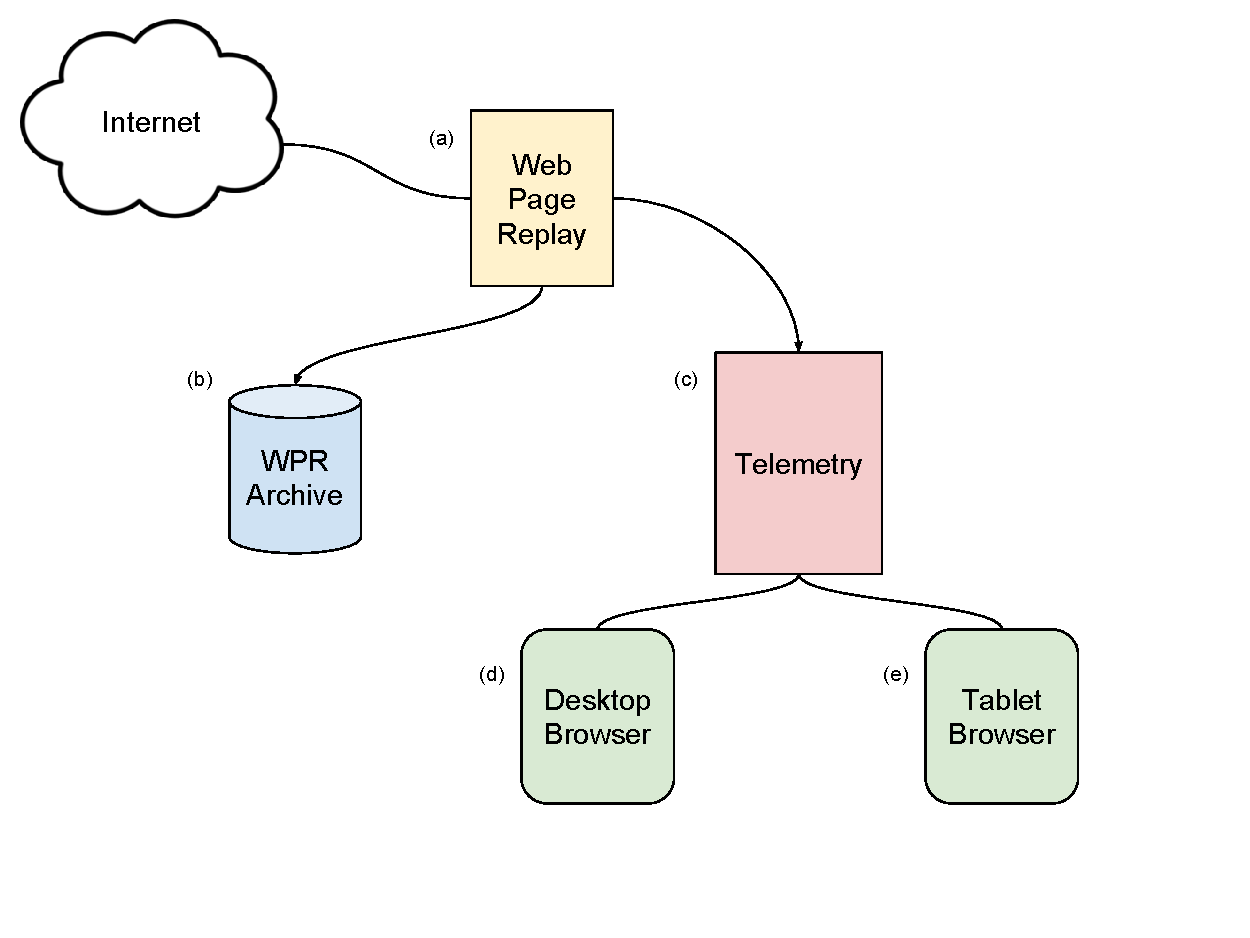
\includegraphics[width=3in]{../images/methodology_workflow_diagram.pdf}
    \caption[]{\label{fig:workflow_diagram}Logical units of our apparatus.}
\end{figure}

\begin{figure*}[!htb]
\hspace{0.01in}
\begin{subfigure}{0.33\textwidth}
    \hspace*{-0.11in}
    \figuretitle{Cacheable Bytes} 
    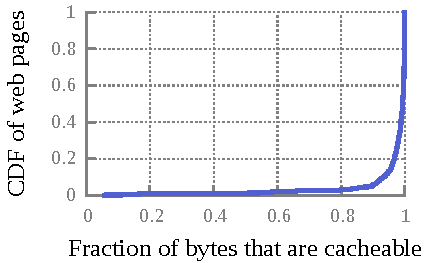
\includegraphics[width=\textwidth]{../graphs/cacheable_bytes/cacheable_bytes_linear.pdf}
    \caption[]{\label{fig:cacheable_bytes_linear}}
\end{subfigure}\hfill
\begin{subfigure}{0.33\textwidth}
    \hspace*{-0.11in}
    \figuretitle{Total Bytes} 
    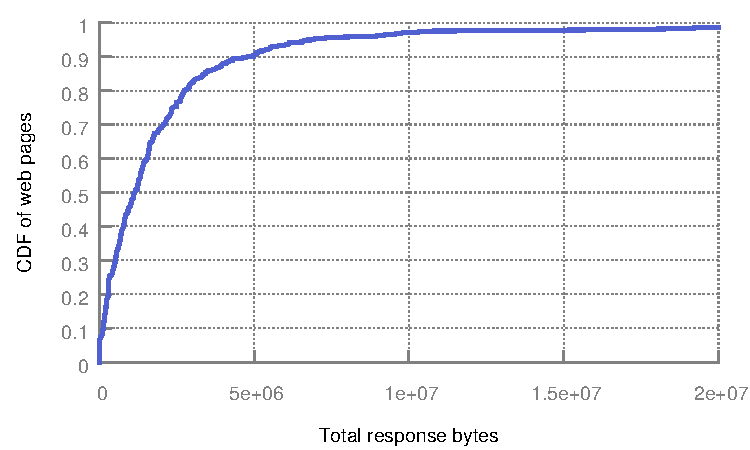
\includegraphics[width=\textwidth]{../graphs/total_bytes/total_bytes_linear.pdf}
    \caption[]{\label{fig:total_bytes_linear}}
\end{subfigure}\hfill
\begin{subfigure}{0.33\textwidth}
    \hspace*{-0.11in}
    \figuretitle{Partial Cache Page Load Time} 
    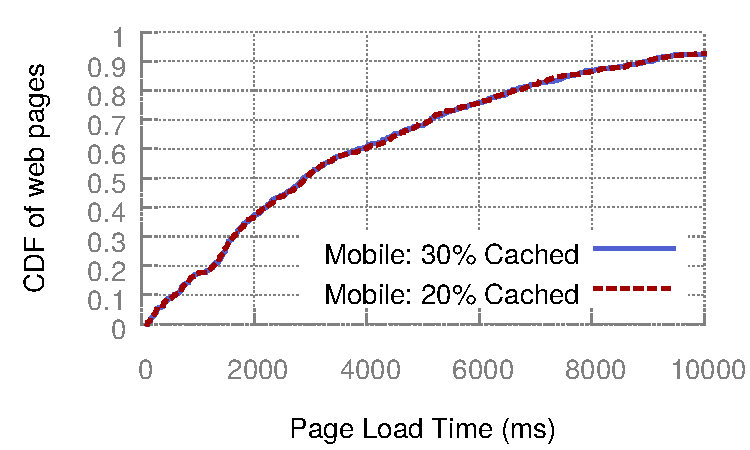
\includegraphics[width=\textwidth]{../graphs/partial_cache/partial_cache_linear_PLT.pdf}
    \caption[]{\label{fig:partial_cache_linear}}
\end{subfigure}\hfill
\caption{(\ref{fig:cacheable_bytes_linear}): The majority of web pages are composed mostly of cacheable bytes. (\ref{fig:total_bytes_linear}): While 95\% of web pages are under 6.8 MB, the median web page size is less than 1.2 MB. (\ref{fig:partial_cache_linear}): Increasing the cache hit ratio from 20\% to 30\% had negligible effects on mobile PLT.}
%\vspace{-0.2em}
\end{figure*}
Before each experiment, we clear the browser cache to ensure consistency across trials. For each device (desktop and mobile), we execute the following steps for each URL:

%\colin{If we're looking to cut space, we might make this more terse, since it's redundant with above}
First, we record the live web page from the Internet using Telemetry to
instruct the browser to fetch the given URL. The WPR proxy receives this
HTTP(S) request, forwards it to the Internet, and passively inspects and
records the two-way traffic as noted in~~\S\ref{setup}. We store this data as
a WPR archive.

Next, we determine the page load time of the web page with a cold cache. With
WPR in replay mode, we load the URL four times (cf.~~\S\ref{known_limitations}) and take the minimum page load time as our PLT value, to account for variance.

Now, we emulate a ``perfect,'' fully populated cache. First, we copy the original WPR archive into a new WPR archive. For each cacheable response in this new WPR archive, we set its network delay to 0 (of course, a ``real" cache response time of 0 is not possible, but we set this as an absolute lower bound). Non-cacheable items, as indicated by HTTP headers, retain their initial network delays. We store this modified archive alongside the original (Figure~\ref{fig:workflow_diagram}b).

Lastly, we record the page load time again, however this time using the modified WPR archive. We determine the PLT in the same way as the original. We then compare the page load times of the unmodified replay executions to that of the modified ``perfect cache'' executions.

\textbf{Partial Caching Methodology}. To confirm Flywheel's findings, we created two additional sets of partially cached WPR archives: one that caches a randomly chosen set of 30\% of all cacheable resources (regardless of byte size), and another that caches 20\%.
We ensure that the cached items in the 20\% WPR archive are a strict subset of the cached items in the 30\% WPR archive for consistency. 
%\arvind{this is the bit which might need justification; why is random the right choice? let us say that I visit cnn.com.  Shouldn't all of the resources inside cnn.com - say js, css, etc. - be either cached or not cached?  Does it make sense for js to be cached and not css?}
%\jamshed{Whole Objects, not bytes, and taking a uniform random distribution}
\subsection{Specifications} \label{specs}
Each web page was originally fetched over UC Berkeley's LAN, which approximates 250 Mbps down and 230 Mbps up.
Our mobile device is a Galaxy Tab 4 with a 1.2 GHz quad-core processor and 1.5 GB on board RAM running Android 4.4, KitKat. Desktop results were performed in a virtual machine with a 3.2 GHz quad-core processor and 6 GB RAM.
%\arvind{maybe this should be pitched as an edge cache?  maybe the fact that this is an edge cache makes the random choice above more palatable?}
\subsection{Known Limitations}  \label{known_limitations}
We identify the following limitations of our apparatus, and discuss the reasoning behind our choice of tools:

%\colin{We can cut this if we need space. Don't really need to defend this choice.}
\textbf{Page Load Time as a Metric}. When determining web page performance, we chose to focus on page load time rather than SpeedIndex~\cite{speed-index} or above-the-fold time~\cite{above-the-fold}.
Although they are arguably preferable metrics (as they do a better job of
capturing the user's perspective), these metrics are significantly more
difficult to measure.% consistently.
%Further, other metrics do not necessarily account for below-the-fold Javascript or other background resources that may cause significant delays to a user's final experience of a web page.

\textbf{WPR Measurement Accuracy}. The PLT measurements taken by WPR are not necessarily consistent with PLTs observed on live web pages, nor are they necessarily consistent across multiple runs of WPR. First, although WPR attempts to mitigate non-determinism in JavaScript execution (by injecting a script into each web page that interposes on non-deterministic calls such as \texttt{getTime}), JavaScript may nonetheless exhibit non-determinism across different loads. Second, the mechanism WPR uses to emulate the original RTTs observed during record mode  (sleeping a fixed number of milliseconds) may not perfectly match the behavior of the original page load.
%These artifacts affect both mobile and desktop browsers in the same manner.
\begingroup
\setcounter{savefootnote}{\value{footnote}}% Store footnote counter
\setcounter{footnote}{2}% Reset footnote counter
\renewcommand{\thefootnote}{1}% Modify footnote printing
We try to mitigate these artifacts by loading each web page four times and
taking the minimum PLT.\footnote{We observed that beyond four loads per web page, the minimum PLT value did not decrease significantly.}
\setcounter{footnote}{\value{savefootnote}}% Restore footnote counter
\endgroup
%\footnote{We observed that beyond four loads per web page, the minimum PLT value did not decrease significantly.}.
%\footnote{We observed that beyond four loads per web page, the minimum PLT value did not decrease significantly.}
%\textbf{WPR Interference}. In our apparatus, the WPR proxy acts as a middlebox between the client and the web content. While we make this proxy transparent, it is possible that it interferes with our experiment. \jamshed{add or remove}.


%\vspace{-0.2in}
\section{Results}
\label{sec:results}
Here, we demonstrate empirical performance results we have found with our
apparatus. We also attempt to highlight the underlying effects that determine
our results.

\subsection{Workload Characteristics}
We first note several key characteristics of our data corpus:

\textbf{Data Set}. We selected a random subset of 400 of the Alexa top 2000 URLs~\cite{alexa} and loaded their root URL (`/').
% \textbf{Cache Hit Ratio}. We experiment with two settings of cache hit ratio. To show an upper bound on how much caching can help, we evaluate the effect of a perfect (100\%) cache. We also seek to reproduce the result from Flywheel~\cite{flywheel}, by showing the difference between 20\% and 30\% cache hit ratio.
% %In their NSDI paper, Google reported that increasing the cache hit ratio by more than 50\% only increased mobile PLT by 1-2\%. Here, we seek to capture an upper bound on caching's effect on PLT. 

\textbf{Fraction of Cacheable Bytes}. Over 90\% of web pages in our workload have more than 90\% of their total bytes marked as cacheable, as shown in Figure~\ref{fig:cacheable_bytes_linear}. %This gives the initial impression that perfect caching should have a significant effect on web performance.
%Web pages generally make high use of caching between origin servers and users.

\textbf{Total Bytes}. Figure~\ref{fig:total_bytes_linear} shows the spread of web page sizes in our data set. While 95\% of web pages are under 6.8 MB, the median web page size is less than 1.2 MB.

\textbf{Initial Network Delays}. Across all requests/response pairs, the median delay between sending the request and receiving the first response byte was 50ms, with a mean of 151.17ms and standard deviation of 403.77ms.
%Initial network delays may play a role in determining the final results of our caching analysis. 
% TODO(cs): we should include this next sentence?!
%As such, we experimented with inflating all network delays by a fixed amount (100ms) to emulate what clients in an emerging market might observe. We found that the mobile results of our caching analysis were changed by 3\% in the median case (See Figure~\ref{fig:inflated_delays}).
%\arvind{this is to the original website right?  the "LAN" is confusing.}

\textbf{User Agent}. Many web pages are now optimized for mobile devices. Web
servers inspect the user agents (UA) of incoming HTTP(S) requests to deliver
customized content to the client depending on their device size and
computational resources. We ran all of our experiments twice: once where the
browsers (both desktop and mobile) advertised a mobile UA, and once where the
browsers advertised a desktop UA. We found that the differences in the results
were comparable. Here, we show only the desktop UA results to make our graphs more readable.
%\arvind{shouldn't it be that the mobile device should use mobile UA and the desktop one should use the desktop UA? the fact that the differences - as opposed to the actual values - are comparable is interesting.} \jamshed{Add slight anecdotal evidence}

\subsection{Performance Results}

As we saw in Figure~\ref{fig:cacheable_bytes_linear}, most pages are composed of a significant number of cacheable bytes. This would seem to suggest that increasing the cache hit ratio should yield a significant improvement in web performance for the end user~\cite{kroeger1997exploring}.

\textbf{Caching Doesn't Significantly Reduce Mobile PLT}.
Similar to Flywheel's result~\cite{flywheel}, we find that increasing the cache hit ratio of a web page does not significantly decrease the user's overall latency on a mobile device.
In fact, with a perfect cache, a mobile device gains only a 13\% PLT reduction in the median case, while its desktop counterpart sees a  PLT reduction of 34\% (see Figure~\ref{fig:percent_reduction_linear}).

Additionally, we emulated partial caches with 20\% and 30\% hit ratios. As shown in Figure~\ref{fig:partial_cache_linear}, we found that increasing the hit ratio by 10 percentage points had negligible effects on mobile page load time. Consistent with Flywheel's NSDI paper, there was only a 1\% reduction in PLT in the median case.

Figure~\ref{fig:ratio_linear_comparison} illustrates how the impact of caching on PLT is limited:
for each 10 percentage point increase in cache hit ratio, there is only a 1 percentage point decrease in mobile page load time.
That is, there is a sharply diminishing marginal performance gain for every additional byte that is cached.
This experiemental evidence supports our model:
the fraction of cacheable bytes on the critical path ($K$) is significantly smaller than the fraction of cacheable byes \textbf{not} on the critical path.

Further, Figure~\ref{fig:plt_cpu_comparison} empirically shows that as CPU speed decreases, the computational time spent processing a web page ($C$) dominates overall PLT, while for faster CPUs, network delays account for most of the PLT ($ C << N $).

\begin{figure}[t]
    %\hspace{-10pt}
    \figuretitle{Ratio of Fraction Cacheable Bytes to PLT}
    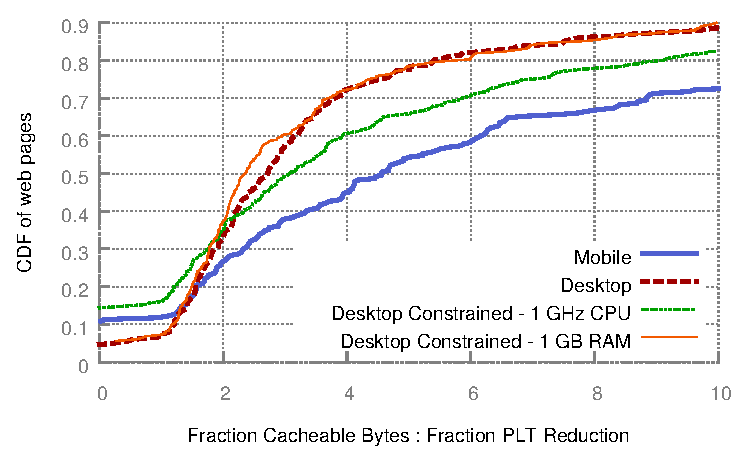
\includegraphics[width=3in]{../graphs/ratio_bytes_to_reduction/ratio_linear_comparison.pdf}
    \caption[]{\label{fig:ratio_linear_comparison}As the percentage of cacheable bytes in a web page increases, the reduction in page load time due to caching increases. However, for each additional percentage cached, there is less than a percentage reduction in page load time.}
\end{figure}
\subsection{Isolating the Difference Between Mobile and Desktop}

% Discuss resource constraints, CPU
We find that the main cause of discrepancy is due to the large difference of CPU speed between desktops and mobile devices. 
We measured this effect by running the same experiment as before, but in virtual machines that were constrained by different resources (using VirtualBox to either set a limit on memory usage or emulate a slower CPU clock speed).
A typical mobile device in the global market today has a 1 GHz processor and 1 GB of RAM~\cite{mobile-stats}. In order to emulate these conditions and isolate computational resources, we restricted one virtual machine to a 1 GHz processor with 6 GB of memory, and another to a 3.2 GHz processor with 1 GB of RAM.

%\colin{Need to also say how much memory/CPU it had, even if if you're focusing on CPU/memory}
In Figure~\ref{fig:percent_reduction_linear}, `Desktop Constrained - 1 GHz CPU' is closely aligned with the results for `Mobile' (our tablet), while `Desktop Constrained - 1 GB RAM' is more closely aligned with the `Desktop' results.
This suggest that CPU is the key difference between caching's effects for mobile and desktop.
In fact, as we throttle CPU constraints, perfect caching has noticeably smaller effects on PLT (See Figure~\ref{fig:plt_cpu_comparison}). Similarly, page load times are generally higher on devices with CPU constraints as seen in Figure~\ref{fig:plt_differences}.

%\colin{Can cut this if we need space}
Consistent with the results found in WProf~\cite{wang2013demystifying}, our results show that reduction in PLT is not proportional to number of bytes cached. We conjecture that the reason mobile performs worse than desktop is precisely because a constrained CPU changes the critical path (when compared to desktop), causing a smaller fraction of the critical path to be network-bound. 
%We hypothesize that the delays of objects on the critical path are also elongated by a constrained CPU.
%These factors contribute to a longer critical path that is prone to the benefits of caching.
%\arvind{above discussion is not clear; and it is probably the most critical observation that we need to communicate precisely}


\subsection{Data Validation}
\label{subsec:validation}
We made several efforts to sanity check the validity our results~\cite{sanity-checks}. To mitigate non-determinism, we compared the status codes of all objects loaded in the browser from both original and perfect/partial cache benchmarks. We filtered out about 9\% of web pages in our 400 URL data set in cases where there were a high number of 404 error codes due to non-deterministic requests without responses in the WPR archive. It is worth noting that the figures we present show only these 91\% of web pages that passed this filter.

As the ratio of cached to non-cached bytes increases in a web page, we expect page load time to be less than or equal to that of its non-cached counterpart. As seen in Figure~\ref{fig:ratio_linear_comparison}, there is a positive correlation between the fraction of cached bytes and the reduction in PLT, albeit asymptotic.
However, due to variance in PLT (discussed in \ref{known_limitations}), we see that a fraction of web pages can perform worse when cached, as seen by points to the left of \texttt{X = 0} in Figure~\ref{fig:percent_reduction_linear}.



\begin{figure}[t]
    %\hspace*{-0.11in}
    \figuretitle{CPU Comparison of PLT Reduction}
    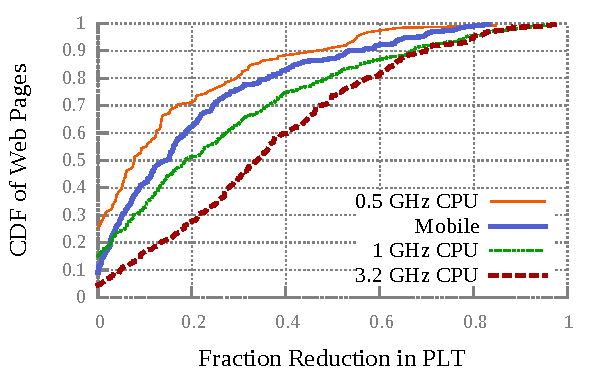
\includegraphics[width=3in]{../graphs/percent_plt_reduction/percent_reduction_linear_CPU_comparison.pdf}
    \caption[]{\label{fig:plt_cpu_comparison}Slower CPU speeds curtail the efficacy of caching to reduce page load time.}
\end{figure}


%\vspace{-0.3in}
\section{Related Work}
\label{sec:related_work}
%Due to the burgeoning interest in web page speed, there has been a recent rise of network caching literature, tools, and companies.

% TODO(cs): explain that in the NSDI'15 slides, we presented a simple critical
% path model, and
% conjectured that objects on the critical path are often not in cache
% (cacheable). However, we didn't have any evidence for this.

Several papers have analyzed web page performance, the effects of caching, and the relationship between CPU speeds and page load time.
% As far as we know, we are the first to jointly isolate all of these factors. % this enables us to easily dissect the effects that caching has on mobile devices.

\textbf{WProf}. Wang et al.~\cite{wang2013demystifying} is the closest research to ours. As we discussed in ~\S\ref{sec:background}, the experiments WProf ran for their Figure 11 show that objects on the critical path are often not cached; and the experiments they ran for their
Figure 13 implies that decreasing CPU speed causes computational delays to comprise a larger fraction of the critical path.

We extend their research along several dimensions.
We develop a model that allows us to predict PLT for a given cache hit ratio. We show that limited RAM does not increase computational delays, though slow CPUs do. We also empirically measure (rather than statically compute, as WProf does) PLTs using a tablet device, and using CPU-constrained virtual machines, over a larger data set (400 URLs, vs. {\footnotesize$\sim$}50 URLs).
Lastly, we extend WProf's cacheability analysis to show that the
marginal returns from caching sharply diminish.

% WProf found that:
%   - Fig 11a & 11b, taken together, seem to imply that objects on the critical
%     path often aren't cached. "cached bytes not proportional to PLT"
%   - Even stronger: Fig 11b shows specifically that while caching reduces 65\%
%     of total object loads, it only reduces 20\% of object loads on the
%     critical path.
%   - Fig 13 seems to imply that decreasing the CPU speed tends to make
%     computational delays dominate over network delays

% Specific ways that we extend their results:
%   - Develop a model, extend their what-if to C=2
%   - Empirically measure slow CPUs, not just what-if. (Fig 7,8,9)
%   - Fig 6 not in WProf (expands on their analysis of K)
%   - Larger dataset: they had at most ~50 URLs, vs. 400 for us.

%\colin{The second and third sentences are too vague.}
\textbf{Web Performance for Desktop}. Related studies~\cite{web-perf-2, web-perf-3} focus on evaluating and optimizing web performance for desktops. Many techniques such as altering content, data compression, proxy services, and CDNs have been exploited to reduce latency for users. These studies focus on high performing end devices such as desktops. We additionally analyzed web performance on a mobile device and show how this differs from classic desktop environments.
%\jamshed{Say something like `the set of assumptions does not hold for mobile.'}

\textbf{Proposed Changes to the Web}. There are many papers~\cite{web-perf-4-new-design, web-caching-4-new-design, web-caching-5-new-design, web-caching-latency-1-new-design, web-caching-latency-2-new-design, web-caching-latency-3-new-design, web-caching-latency-5-new-design, web-caching-latency-6-new-design, web-caching-latency-7-new-design} that propose changes to the web that would improve latency for both desktop and mobile devices through better caching schemes. It is possible that under their proposed changes, caching would have more of a benefit for mobile latency. In this paper, we focus only on today's existing browser infrastructure. % We further show that increasing the hit ratio of caches only provides marginal benefits to mobile page load time.

%\colin{This is very exciting! If there are papers that claim that caching should help mobile latency, we're showing that they're wrong! We need to emphasize this much more!}
\textbf{Web Caching}. Other literature~\cite{web-caching-1, web-caching-2, web-caching-8, web-caching-9} has focused on the benefits of web caching, specifically the reduction of latency for desktops~\cite{web-caching-3, web-caching-4, web-caching-5, web-caching-6, web-caching-7}.
While these papers make note of the several benefits of caching, their set of assumptions do not necessarily hold for mobile devices, which have significantly less computational power. 
% Good.

\textbf{Mobile, CPU Speeds, and PLT}.
Some research has also investigated the extent to which CPU speed determines page load time, for desktop~\cite{CPU-plt-1} and mobile devices~\cite{CPU-plt-2, CPU-plt-3}.
%Research has also been conducted regarding the correlation between CPU speed and page load times. Jones et al. ~\cite{CPU-plt-1} noted that increased page load time on mobile devices was due to the lack of CPU power, but did not provide backing evidence.
Zhen Wang et al.~\cite{CPU-plt-2, CPU-plt-3} have determined that the largest delay factor in desktop web page loading is object rendering in the browser. They went further to show that CPU constraints are the lead cause of slow resource loading.
With a large data set, we bolster the claim that suggests that CPU constraints are the critical factor in determining page load time. We also demonstrate that web caching has diminishing benefits due to the limited CPU speeds of mobile devices.

%\jamshed{TODO: discuss other methodologies, why is our apparatus novel?}
% \jamshed{From Colin: Most other papers measure results "in the wild", i.e. on real networks. That's useful for the final results, but it's hard to control it well enough to get repeatable results.}
%\begin{figure}[t]
%    %\hspace{-10pt}
%    \figuretitle{Fraction Reduction in PLT with Inflated Delays}
%    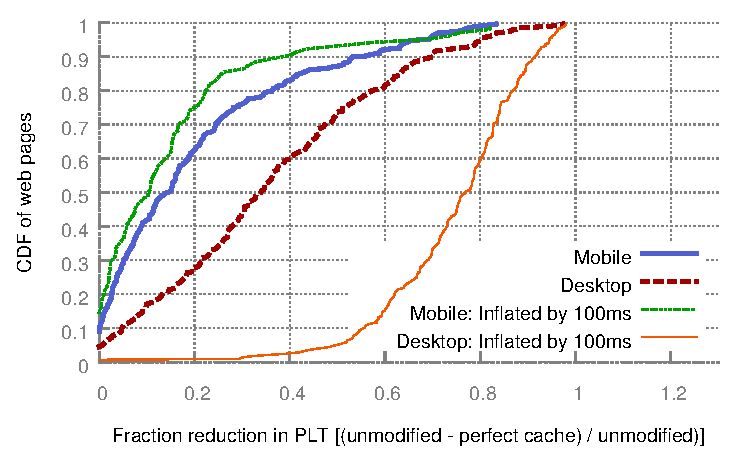
\includegraphics[width=3in]{../graphs/percent_plt_reduction/percent_reduction_linear_inflated.pdf}
%    \caption[]{\label{fig:inflated_delays}In networks with high latency, caching has a negligible effect on mobile PLTs, but a significant benefit for desktop PLTs.}
    % Just remove the first sentence of the caption?
%\end{figure}



%\vspace{-0.3in}
\section{Conclusion}
\label{sec:conclusion}
We have presented an experimental apparatus for examining the effects of caching on mobile page load time.
Using this apparatus, we demonstrate that mobile page load time is not significantly reduced by caching, contrary to common wisdom.
We go further to show that resource constraints, specifically the CPU, appears to be the main difference between caching's effect on desktop versus mobile.
Content providers may want to reconsider where they focus their optimization efforts, especially as mobile traffic begins to outpace its desktop counterpart.

In future work we plan to measure the critical path on mobile devices, experiment with other web page load time metrics, further levels of caching, and inflating the original network delays to better emulate mobile devices in congested network environments. 

Going forward, mobile devices are becoming increasingly powerful and the bottleneck resources will shift. At what point will web caching have a larger benefit for mobile?  

%\subsection{Future Work}
%There is still space to explore these findings. Using other metrics such as above-the-fold PLT and SpeedIndex may provide deeper insight into the reasoning behind limited mobile PLT reduction. Similarly, examining changes in the critical path with a tool such as WProf would provide valuable insight (WProf does not currently have a mobile tool). 

%It is also worth experimenting with varying levels of caching, namely 22\% and  32\% as in the Google NSDI paper~\cite{flywheel} to see if such incremental changes to mobile PLT are observed. \jamshed{Remove if done.}

%Finally, it is worth adding fixed delays to network responses in order to better emulate mobile and congested networks.

%\clearpage

%\vspace{-0.3in}
% \begin{appendices}
% \section{Appendix}
% \appendix
\section{Model Derivation}
\label{sec:appendix}

% Not sure where this content goes yet... but here's an explanation....
Here we derive the page load time performance model stated in~\ref{subsec:model}. We
develop a continuous probability model (i.e., we assume that the size of all
objects sums to 1.0), since we are not aiming for a high degree of accuracy,
and since discrete models are more unwieldly.

%This model is useful for those determining how many resources (money, effort, time, etc) to put into developing an effective cache (such as a CDN).
%That is, with our model, one can estimate the return on investment that is gained by caching.

We introduce one term in addition to those in~\ref{subsec:model}:

\noindent--Let $K$ denote the fraction of objects that are on the critical path.

In our derivation we override the terms $X$ and $K$ to also denote random
variables: the event that a given object is cached and the event that a given
object is on the critical path, respectively.

We make two simplifying assumptions in deriving our model. First, we assume that the probability that an
object is present in the cache is independent of the probability that the
object is on the critical path.\footnote{
This first assumption is likely overly conservative; Figures 11a and 11b of the
WProf paper seem to indicate that objects on the critical path may have lower
probability of being cacheable than other objects~\cite{wang2013demystifying}.}
Second, we assume that the critical path does not change as we vary the cache hit
ratio. That is, we treat $K$ as a constant.

We categorize all objects on the critical path into two distinct groups.
The first category is the fraction of all objects on the critical path that are cached (these
will incur 0 network delay, assuming that the cache is colocated with the
browser):

\begin{align*}
Pr(X|K) & =  Pr(X) & \text{[since $X$ and $K$ are independent]} \\
& = X &
\end{align*}

The second category is the fraction of all items on the critical path that are not cached (these will incur their original network delay):

\begin{align*}
Pr(1-X | K) & = Pr(1-X) & \text{[since $X$ and $K$ are independent]} \\
& = 1-X &
\end{align*}

At a given cache hit ratio $X$, the expected value of the total network delay
on the critical path is (assuming that a cached item incurs zero network delay):
\begin{align*}
E_N[X] & = Pr(X|K) \cdot 0 + Pr(1-X|K) \cdot N \\
& = (1 - X) \cdot N
\end{align*}

Thus, the total expected PLT given a hit ratio $X$ is:
\begin{align*}
E_{PLT}[X] & = C + E_N[X] - f(C,N,X) \\
& = C + (1 - X) \cdot N - f(C,N,X)
\end{align*}

% TODO(cs): To generalize this model to a case where the cache is located far away from
% the browser... we could introduce a non-zero fetch cost associated with
% cached items.

% \end{appendices}
\clearpage

%\vspace{-0.3in}
%\section{Bibliography}
%\label{sec:bibliography}
\bibliographystyle{unsrt}
\bibliography{bib}

\end{document}
